\chapter{Arquitetura Desenvolvida}

O principal objetivo desta dissertação passa pelo desenvolvimento de uma arquitetura que permita a agregação de diversos tipos de dados provenientes de diferentes tipos de sensores colocados de forma distribuída. Para tal foi necessário definir uma forma de ligação uniforme para que todos os tipos de sensores se conectassem à plataforma, bem como um \textit{standard} de comunicação de dados proveniente dos nodos da arquitetura. Foi ainda desenvolvida uma camada de persistência responsável por registar a informação em bruto e processada, sendo esta última o resultado do processamento dos dados levantados pelos serviços de métricas integrados na plataforma. A arquitetura é também responsável pela gestão dos serviços que se encontram a ela ligados.

\begin{figure}[htb]
   \centering
   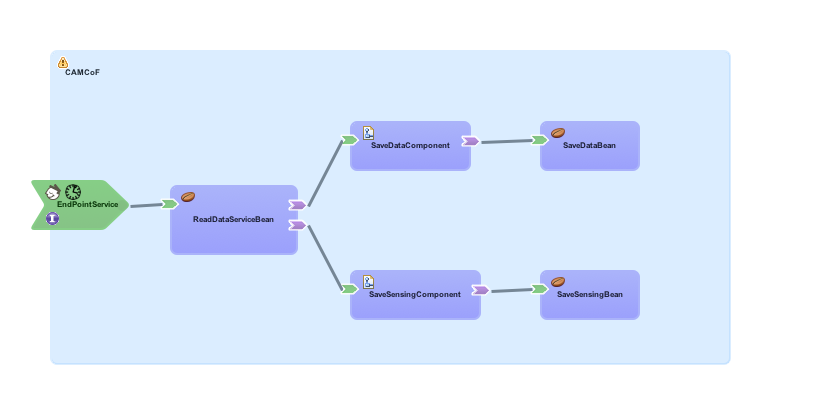
\includegraphics[scale=0.55]{Images/switchyard.png}
   \caption{Diagrama do SwitchYard com os componentes da arquitetura}
\end{figure}

\section{Interoperabilidade}

O desenvolvimento desta arquitetura está assente num princípio fundamental que se baseia em garantir a interoperabilidade de diferentes componentes. Com base neste princípio foram definidos e implementados métodos que permitem que diversos tipos de sensores possam efetuar de forma eficiente a sua ligação à arquitetura e assim contribuir para um correto funcionamento da plataforma. Posto isto é possível garantir não só uma comunicação transparente entre os diversos dispositivos, bem como uma troca efetiva de informação e permitir que novos sensores possam ser adicionados à arquitetura.

Antes de explicar em pormenor como é que esta arquitetura garante a interoperabilidade dos seus componentes, importa definir exatamente em que consiste a interoperabilidade e o que define um sistema com esta característica. Assim, a interoperabilidade é capacidade de diversos componentes comunicarem de forma transparente garantindo a cooperação entre eles. Estes componentes tem, em várias situações, origens tecnológicas e características bastante diferentes, o que leva a necessidade de definição de padrões de comunicação abertos e com recurso a linguagens e protocolos comuns(citação). Num sistema interoperável, como a arquitetura desenvolvida, todos os seus componentes devem então, independentemente da sua diversidade e definição tecnológica, ser capazes de cooperar e comunicar de forma clara e transparente através da definição de padrões e normas necessárias. A arquitetura implementada através dos padrões de comunicação definidos permite também a adição de forma automática de novos componentes, podendo estes acrescentar, através das suas funcionalidades, valor à arquitetura.(citações)

Posto isto, o método de ligação dos sensores, que podem ser vistos como os nodos da arquitetura responsáveis pela recolha de dados, à arquitetura foi definido de modo a garantir este conjunto de pressupostos apresentado. Foi então padronizado que os novos nodos para efetuarem a sua ligação à arquitetura devem enviar uma mensagem com um objeto JSON através do método POST para o seguinte endereço URL:

http://127.0.0.1:8080/CAMCoF/send/connect

O objeto a enviar pelo sensor que pretende conectar-se à arquitetura deve conter um conjunto de informações sobre o sensor de modo a que a arquitetura o consiga identificar e registar como um novo sensor da arquitetura. O objeto JSON deve assim conter o identificador do utilizador fornecido no momento de registo do utilizador na interface desenvolvida para a arquitetura, um endereço de comunicação do serviço para o qual a unidade central da arquitetura possa comunicar, um identificador do sensor, o tipo de serviço de monitorização oferecido pelo sensor, a frequência de comunicação de dados, o tipo de dados a enviar e ainda uma descrição do serviço.

\begin{lstlisting}[caption=Exemplo de objeto JSON enviado por Sensor de Teclado]
{
  "id": "1236",
  "ip": "23.254.109.135:999/keyboard/com",
  "type":"keyboard",
  "sensorid":"00:01:29:D3:95:C6",
  "period":"10",
  "typedata": "string",
  "description": "Keyboard Sensor Model A15526"
}
\end{lstlisting}

A unidade central perante a informação recebida inicia um processo de verificação da informação. Em primeiro lugar verifica se o identificador do sensor recebido corresponde a um sensor já utilizado na arquitetura, se não for este o caso o novo sensor será registado. Deste modo existe apenas um registo por cada sensor utilizado na arquitetura independentemente da sua utilização em vários momentos e do utilizador em questão. De seguida é registado o novo nodo da arquitetura, definido essencialmente pelo endereço de comunicação e pelo registo do sensor utilizado. Por fim, é criado o registo de monitorização ao qual serão associados os vários registos posteriormente levantados e enviados pelo nodo em questão.

\begin{figure}[htb]
   \centering
   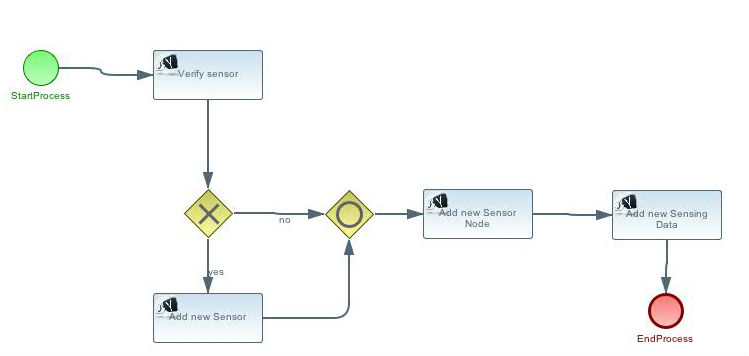
\includegraphics[scale=0.55]{Images/SaveSensingComponent.jpg}
   \caption{BPMN de conexão à arquitetura}
\end{figure}

Concluído este processo é enviada uma resposta ao pedido de conexão. Em caso de sucesso do pedido, independentemente do sensor já se encontrar registado previamente na arquitetura ou não, o novo nodo receberá como resposta um objeto JSON que será composto por um código de confirmação da integração do serviço na arquitetura e por um endereço através do qual o sensor deverá comunicar os dados a recolher durante a monitorização.\\

\begin{lstlisting}[caption=Mensagem de sucesso em JSON]
{
	"status":"200"
	"url":"http://127.0.0.1:8080/CAMCoF/send/1236/00:01:29:D3:95:C6"
}
\end{lstlisting}

No caso de se verificar algum problema com os dados enviados na mensagem de conexão à arquitetura, como por exemplo o identificador do utilizador não existir, ou de este nodo já se encontrar registado na arquitetura, a resposta obtida será uma mensagem a reportar o conflito ocorrido.\\

\begin{lstlisting}[caption=Mensagem de conflito em JSON]
{
	"status":"409"
	"url":"Conflict - Service already exists"
}
\end{lstlisting}


\section{Comunicação de Dados}

Definido o método de ligação dos nodos da arquitetura, importa estabelecer a forma como os dados recolhidos pelos sensores são enviados para a unidade central onde serão posteriormente tratados e armazenados. A comunicação da informação implementada na plataforma pretende garantir um método simples e fiável de transmissão dos dados de modo a que a informação possa ser gerida na unidade central. O feedback desta operação é também comunicada ao nodo da arquitetura responsável pela recolha da informação, para que este possa saber o estado deste processo em particular.

Na sequência do método implementado para a ligação dos nodos que compõem a arquitetura e de forma a garantir também os parâmetros básicos definidos para a comunicação da informação, esta operação estará exclusivamente disponível para os nodos conectados através do seguinte seguinte endereço URL:

http://127.0.0.1:8080/CAMCoF/send/id\_utilizador/id\_sensor

Este endereço foi definido de acordo com as informações registadas para cada nodo da arquitetura. Isto é, para cada nodo o \textit{id\_utilizador} irá corresponder ao identificador do utilizador registado na plataforma e o \textit{id\_sensor} ao identificador do sensor utilizado, informação essa registada no processo de conexão à arquitetura e já apresentado neste capítulo.

Relativamente aos dados a enviar estes são enviados sob a forma de uma String através do método POST. O exemplo abaixo representa um pequeno excerto de um registo de dados levantado por um sensor de movimento do rato sob a forma de uma String, que foi posteriormente enviada para a unidade central da arquitetura.\\
\begin{lstlisting}[caption=Excerto de dados levantado por sensor de movimento de rato]
MOV,63526767801398,None,599,36
MOV,63526767801404,None,600,36
MOV,63526767801416,None,601,36
MOV,63526767801436,None,601,36
MOV,63526767801480,None,602,36
MD,63526767801725,Left,602,36
MU,63526767801925,Left,602,36
\end{lstlisting}


Tendo em conta que este processo de comunicação da informação levantada pelos sensores é fundamental para o funcionamento da arquitetura, importa garantir que nenhum registo é perdido neste processo de comunicação. Posto isto, foi definido uma resposta padrão enviada pela unidade central para o nodo responsável pelo envio da informação dando conta do sucesso da operação. Assim, apenas no momento da receção dessa resposta o nodo poderá registar esse processo como concluído e avançar para a tarefa seguinte. Caso esta resposta não chegue, o nodo deve reenviar os dados para que esta possa ser registada. Abaixo apresenta-se o objeto JSON enviado pela unidade central dando conta do sucesso da operação de comunicação, como o próprio código presente no objeto indica.\\

\begin{lstlisting}[caption=Mensagem de sucesso em JSON]
{
	"code":"200"
}
\end{lstlisting}


Se a tentativa de comunicação for efetuada por um serviço que não se encontre, no momento, ligado à arquitetura o objeto de resposta contém o código 403, informando que este não tem permissões para estabelecer essa comunicação.


\section{Registo de Informação em bruto}

A informação recolhida pelos sensores que constituem a arquitetura deve ser armazenada para que seja possível, posteriormente, tratar os dados e retirar conclusões sobre estes. Deste modo, a informação que os sensores registados e conectados na arquitetura vão enviando para a unidade central é armazenada na base de dados antes de se iniciar qualquer tipo de operação sobre os dados. Nesta fase os dados são armazenados exatamente como foram registados pelos sensores, pelo que os registos correspondentes podem mais tarde ser consultados.

O armazenamento da informação em estado bruto na base de dados da plataforma representa  o primeiro nível de armazenamento de dados definido para o registo de informação proveniente dos sensores. Desta forma é possível ter, em qualquer momento, acesso à informação em bruto, caso esta seja necessária, avançando-se somente de seguida para o processamento dos dados com o recurso a serviços de métricas. 

O método de armazenamento dos dados implementado pretende assim o registo na base de dados da informação à medida que esta é enviada pelos nodos, em diferentes estados de tratamento, sendo esta primeira fase o início de um processo ao qual se segue o processamento da informação e posteriormente um novo registo da informação num outro nível. O objetivo deste método consiste em retirar o máximo de proveito da informação recolhida sobre o comportamento e ambiente em que o utilizador da arquitetura se encontra envolvido. 

\begin{figure}[htb]
   \centering
   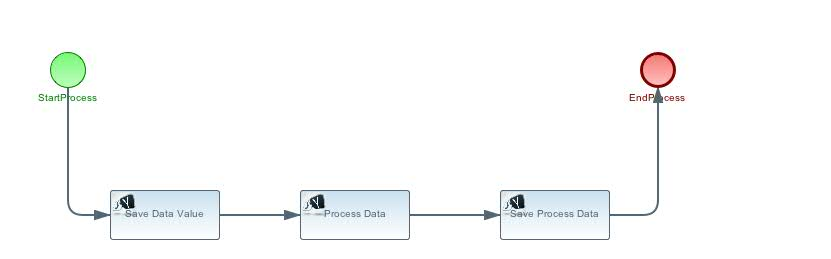
\includegraphics[scale=0.6]{Images/SaveDataComponent.jpg}
   \caption{BPMN de armazenamento da informação enviada pelos sensores}
\end{figure}

\section{Integração de Serviços de Métricas}

Os dados enviados pelos sensores para a unidade central e armazenados na base de dados em bruto são processados por um conjunto de serviços de métricas integrados na arquitetura, dando origem a um nível de informação mais refinado, sobre o qual se pretende conseguir retirar conclusões concretas. Os diversos serviços de métricas permitem que os dados recolhidos por um sensor de determinado tipo seja submetido a um processamento específico tendo em conta a sua origem. O resultado da execução dos serviços de métricas é novamente reencaminhado para a unidade central da arquitetura para que possa ser armazenado.

Assim à medida que os sensores recolhem informação e a encaminham para a unidade central, os dados recebidos são armazenados em bruto, tal como já foi explicado neste capítulo. De seguida, sempre que os serviços de métricas estejam disponíveis, são enviados para os serviços de métricas para que estes possam processá-los. Importa então sublinhar a forma como estas métricas foram desenvolvidas e integradas na arquitetura, bem como o valor que acrescenta ao seu funcionamento e ainda apresentar os diversos tipos de métricas existentes e a forma como estes se relacionam com os dados em bruto recolhidos.

\subsection{Desenvolvimento de Métricas}

\subsection{Tipos de Métricas - acabar preencher}

Os serviços de métricas disponíveis na arquitetura estão diretamente relacionados com o tipo de sensor responsável pela recolha de informação. Desta forma, para cada registo recolhido por um sensor, este poderá ser processado por diversas métricas desse tipo de dados, obtendo-se como resultado um registo correspondente a cada serviço de métrica utilizado. Cada métrica terá um foco específico, sendo o resultado obtido um registo do comportamento do utilizador nesse aspeto em concreto.

Posto isto, foram integrados na arquitetura um conjunto de tipos de métricas que pretendem  complementar a capacidade de agregação de informação da arquitetura, permitindo que esta possa ser analisada sob vários parametros e de diferentes formas. De seguida são então apresentados os tipos de métricas integradas na arquitetura neste momento, uma pequena descrição de cada métrica e ainda o tipo de dados a que cada uma se encontra associado.

\begin{center}
    \begin{longtable}{ | p{4cm} | l | p{7cm} |}
    \hline
    Nome & Tipo Dados & Descrição \\ \hline
    Key Down Time & Teclado & Tempo durante o qual uma tecla é pressionada. \\ \hline    		    Time Between Keys & Teclado & Tempo percorrido entre duas teclas pressionadas. \\ \hline
    Mouse Velocity & Rato & A distância percorrida pelo rato em pixels por intervalo de tempo, em milisegundos. \\ \hline
    Mouse Acceleration & Rato & A velocidade do rato em pixels/milisegundo por intervalo de tempo, em milisegundos. \\ \hline
    Time Between Clicks & Rato & Tempo percorrido entre dois cliques do rato. \\ \hline
    Double Click Duration & Rato & Tempo percorrido entre dois cliques seguidos, sempre que esse valor for inferior a 200 milisegundos. \\ \hline
    Average Excess of Distance & Rato & Calcula o excesso de distância médio percorrido durante um clique do rato. \\ \hline
    Average Distance of the Mouse to the Straight Line & Rato & Calcula a distância média percorrida em linha reta definida pela localização de dois cliques consecutivos. \\ \hline
    Distance of the Mouse to the Straight Line & Rato & Calcula a distância percorrida em linha reta definida pela localização de dois cliques consecutivos. \\ \hline
    Signed Sum of Angles & Rato & Pretende determinar se o movimento do rato tende a desviar mais para a direita ou para a esquerda. \\ \hline
    Absolute Sum of Angles & Rato & Pretende quantificar o desvio do movimento do rato independentemente da sua direção. \\ \hline
    Distance Between Clicks & Rato & Representa a distância total percorrida entre dois cliques consecutivos. \\ \hline
    Click Duration & Rato  & Tempo percorrido entre pressionar e levantar em cada clique do rato. \\ \hline
   Distance During Clicks &  Rato &  Distância total percorrida entre pressionar e levantar em cada clique do rato.\\ \hline
   Excess of Distance Between Clicks & Rato  & Calcula o excesso de distância percorrido entre dois cliques do rato. \\ \hline
   Pause Use & Rato/Teclado  & Calcula o número de vezes que o rato/teclado não é utilizado. \\ \hline
   Writing Velocity & Teclado  & O número de teclas pressionadas por intervalo de tempo. \\ \hline
   Writing Acceleration & Teclado  & A velocidade do rato por intervalo de tempo. \\ \hline
    \end{longtable}
\end{center}



\section{Comunicação com Serviços de Métricas}

Os serviços de métricas integrados são externos à arquitetura, contudo prestam um serviço bastante importante para o seu funcionamento. Através do método de comunicação estabelecido entre a unidade central da arquitetura e os diversos serviços de métricas, estes recebem os registos em bruto recolhidos pelos sensores e retornam esses dados processados de acordo com as métricas implementadas.

A comunicação estabelecida entre os serviços de métricas e a unidade central da arquitetura, baseia-se mais uma vez no envio de uma String correspondente aos dados registados na arquitetura, através do método POST. Tal como já foi referido, cada tipo de dados permitirá a utilização de um conjunto de métricas com as quais está relacionado. Desta forma, é também nesta fase que é feita a associação entre o tipo de sensor a que correspondem os dados recolhidos e consequentemente filtrado o conjunto de serviços de métricas a utilizar. Posto isto, são enviados os dados a processar para esse conjunto de métricas através do método de  comunicação descrito.

\begin{figure}[htb]
   \centering
   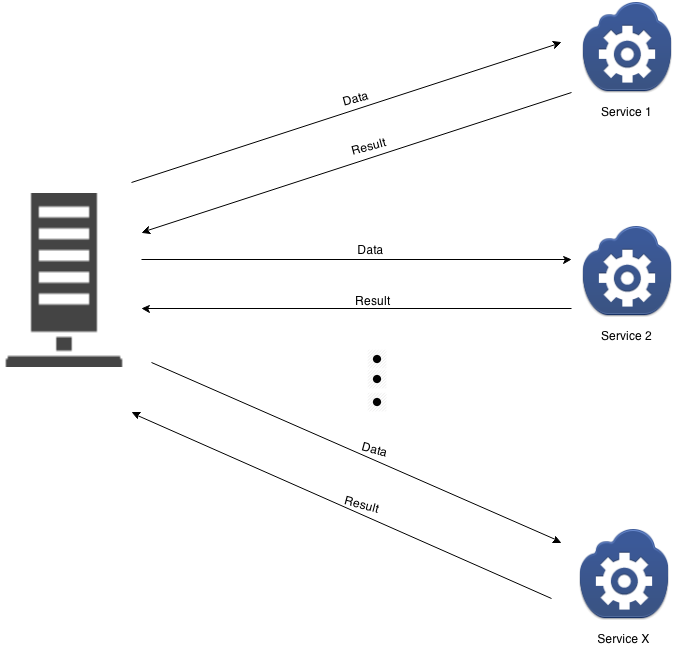
\includegraphics[scale=0.5]{Images/metricsdiagram.png}
   \caption{BPMN de armazenamento da informação enviada pelos sensores}
\end{figure}

Como resultado do processamento dos dados enviados cada serviço de métrica retorna um valor correspondente ao \textit{input} submetido. Estes dados processados de acordo com as métricas implementadas correspondem a um nível de informação mais refinado do que o anteriormente submetido. Sendo também este registado na base de dados da aplicação para posterior utilização.

\section{Registo de Informação Processada}

O registo da informação resultante da utilização dos serviços de métricas integradas na arquitetura corresponde a um nível de dados superior relativamente aos dados em bruto armazenados numa fase anterior. O armazenamento dos dois estados dos dados garante não só a consulta dos dados em bruto caso seja necessário, como garante que caso os serviços de métricas não estejam disponíveis em determinado momento, os dados possam ser submetidos para os serviços correspondentes posteriormente.

Este estado da informação é então armazenado na base de dados da aplicação, tal como no caso da informação em bruto, à medida que os serviços de métricas vão respondendo com a informação processada. Esta informação é armazenada como correspondente a um segundo nível de informação, que indica que esta se encontra refinada comparativamente ao primeiro nível, os dados em bruto. Nesta fase a informação registada pode ser agora utilizada como indicador de ocorrência de estados como fadiga ou stress por parte dos utilizadores da arquitetura.

\section{Verificação de Serviços Conectados}

A arquitetura pode em cada instante ter vários sensores conectados a recolher informação para a unidade central. Dada esta situação torna-se relevante haver um controlo sobre o estado em que se encontra cada um dos sensores ligados ao longo do tempo. Com esse intuito e de forma a haver uma gestão eficiente dos nodos da arquitetura foi pensada e desenvolvida uma forma de gerir e controlar o estado destas ligações com o decorrer do tempo.

Assim, tal como já foi abordado neste capítulo, à medida que cada sensor estabelece uma ligação à arquitetura, essa ligação para além de registada na base de dados, é também armazenada dinamicamente como um sensor que nesse instante se encontra ligado à arquitetura a recolher e transmitir novos dados. É sobre esse registo dinâmico que deve ser feito o controlo de ligação ao longo do tempo, para prevenir situações em que por algum motivo, ocorra um problema com um sensor e este pare de comunicar ou recolher informação, ou simplesmente termine o seu período de monitorização.

Para controlar a ocorrência destas situações foi estabelecido uma comunicação periódica entre a unidade central e todos os sensores que se encontram conectados nesse momento, de modo a confirmar se estes se mantém ligados à arquitetura. Para tal é enviada uma mensagem JSON através do método POST, para cada um dos nodos, na qual é indicado o identificador do utilizador, o identificador do sensor em questão e que se trata de um pedido de informação sobre o seu estado.\\

\begin{lstlisting}[caption=Mensagem de verificação de estado de um nodo]
{
	"id" : "1236",
  	"sensorid" : "00:01:29:D3:95:C6",
	"status" : "request"
}

\end{lstlisting}

O endereço de comunicação utilizado é o endereço URL fornecido por cada serviço no momento da conexão à arquitetura. Como resposta cada nodo deverá enviar um objeto JSON semelhante, contendo o atributo \textit{status} o código 200 caso este pretenda confirmar a permanência da conexão ou o código 410 caso esta pretenda terminar a ligação. Pode ainda ocorrer um terceiro cenário, no qual o nodo não responda em tempo útil, dando-se uma situação de \textit{timeout}, sendo o nodo eliminado da lista de serviços conectados nesse momento.

Todo este processo de verificação de serviços ligados à arquitetura é repetido de forma frequente e periódica pela arquitetura para garantir que não existe um acumular de serviços que já terminaram o seu período de monitorização, sem que a unidade central tenha conhecimento disso e possa por em causa o correto funcionamento da arquitetura.

\section{Cenários de Utilização}

Existe um vasto conjunto de cenários em que a arquitetura descrita neste capítulo pode ser utilizada e revelar-se extremamente útil. Esta arquitetura dada as suas caraterísticas pode, por exemplo, ser utilizada em diversos cenários em que se pretende analisar variações comportamentais e de performance em ambientes profissionais ou de teste. Os resultados obtidos podem também ser utilizados para deteção de situações como fadiga ou stress. Na sequência destas possibilidades os registos e comportamentos monitorizados podem ser utilizados para encontrar formas que levem à diminuição de ocorrência destes fatores em determinadas situações e promover assim o bem estar dos seus utilizadores.

Relativamente a cenários de utilização em concreto podem ser apontados vários. Um exemplo que revela a utilidade e potencial deste trabalho é a utilização da arquitetura na monitorização dos empregados de uma empresa. Neste caso podem se recolhidas informações sobre o comportamento de todos os empregados e fazer análises comparativas e individuais da performance e comportamento com o intuito de encontrar formas de potencializar o rendimento dos seus empregados. Outra situação em que a arquitetura pode ser utilizada é na monitorização de jogadores de computador, podendo recolher informação sobre o seu comportamento e situações que levem a alterações de comportamento ou sinais da ocorrência de stress. A monitorização da reação de indivíduos ao ouvirem determinado tipo de música é outro cenário muito interessante para a utilização da arquitetura dado que permite registar a forma como cada um reage perante diferentes estilos e músicas. O que permite retirar conclusões que podem ser utilizadas em diversas áreas.

Os vários cenários de utilização descritos são apenas exemplos dum vasto leque que compravam a utilidade desta arquitetura e demonstram o potencial que esta revela em áreas extremamente diversificadas. Isto constata que esta solução poderá ter um contributo importante e de grande utilidade em vários contextos.

\section{Conclusão}

O principal objetivo da arquitetura desenvolvida, tal como já foi abordado, consistia na construção de uma arquitetura que permitisse a recolha de informação através da utilização de sensores colocados de forma distribuída. Assim os sensores seriam capazes de monitorizar o comportamento dos utilizadores e permitir que esses dados fossem armazenados para posterior utilização e análise. Este objetivo, através das etapas percorridas e apresentadas neste capítulo, foi alcançado. A arquitetura desenvolvida permite que os seus utilizadores usem diversos dispositivos de recolha de informação, em diversos locais, contextos diferentes e fontes de informação diversificadas também. Através da utilização desta arquitetura, os seus utilizadores têm garantias de fiabilidade e estabilidade de todo o sistema e ainda métodos de comunicação que garantem o correto funcionamento da arquitetura, bem como o armazenamento dos dados recolhidos.

Uma das decisões tomadas, que teve grande influência no desenvolvimento da arquitetura, e que importa mais uma vez sublinhar foi a escolha da \textit{framework} SwitchYard para implementar a arquitetura. Esta decisão revelou-se extremamente sensata pois o potencial identificado na análise feita à \textit{framework} acabou por se verificar e foi bastante útil durante o período de desenvolvimento. O SwitchYard, orientado para o desenvolvimento de aplicações orientadas a serviços, permitiu, através do vasto leque de componentes que dispõe, definir um design e implementação da comunicação entre os nodos da arquitetura e a unidade central e desenvolver ainda as funcionalidades exigidas para essa unidade. Todo o processo de desenvolvimento beneficiou da utilização da \textit{framework}, podendo-se inclusivamente afirmar que este se revelou mais simples, orientado e rápido graças a este.

Outro dos aspetos a salientar nesta arquitetura é a sua comunicação e a forma como esta é estabelecida nas várias tarefas executadas ao longo de todo o processo ao qual a informação recolhida é sujeita. Os métodos de comunicação estabelecidos e implementados permitem garantir que todo o fluxo pelo qual a informação passa seja efetuado de forma eficiente e fiável. O cuidado no desenho destes métodos de comunicação teve ainda por base garantir a interoperabilidade de todos os componentes da arquitetura. Deste modo, é possível afirmar que a arquitetura oferece aos seus utilizadores a capacidade de utilizar diversos tipos de sensores sem que isto coloque em causa o seu correto funcionamento. Cada utilizador pode assim recorrer aos sensores que entender, dado que os métodos de comunicação implementados permitem uma ligação eficiente destes dispositivos e a sua cooperação na execução das suas tarefas no contexto da arquitetura.

De referir ainda a utilização dos serviços de métricas e do valor que acrescentam à arquitetura e ao serviço que oferecem aos seus utilizadores. Estas permitem que os dados recolhidos sejam refinados para um nível perceptível por parte dos utilizadores. Para além disso abrangem vários aspetos do comportamento do utilizadores monitorizados e permitem ter uma noção real dos registos e variações ocorridos ao longo do período de monitorização. Esta panóplia de informação que a arquitetura consegue oferecer, para determinados tipos de dados, acrescenta bastante valor à arquitetura. Para além disso, o método de comunicação e integração dos serviços de métricas está implementado de forma a que seja possível facilmente agregar e disponibilizar novos serviços de métricas, bastando para isso que estes novos serviços sejam registados na base de dados da arquitetura.

